\documentclass{beamer}

\mode<presentation>{
\usetheme{PaloAlto}
%\usetheme{Berlin}
\usecolortheme{default}
\usefonttheme{professionalfonts}
}

\usepackage[utf8]{inputenc}
\usepackage[ngerman]{babel}
\usepackage{graphicx}
\usepackage{booktabs}
\usepackage{svg}
\usepackage{url}
\usepackage{appendixnumberbeamer}
\usepackage{subfigure}
\usepackage{hyperref}

\usepackage{physics}
%\usepackage{relsize}
\usepackage{amsmath}
\usepackage{commath}
\usepackage{xfrac}
\usepackage{xcolor}

\title{Spektralfunktion der single-impurity DMFT mit Hilfe exakter Diagonalisierung für das Hubbard-Modell}
\author{Christoph Gäntgen}
\institute[]{Physikalisches Institut\\
	Rheinische Friedrich-Wilhelms-Universität Bonn}
\date{10. Januar 2019}


\makeatletter
\setbeamertemplate{sidebar \beamer@sidebarside}%{sidebar theme}
{
	\beamer@tempdim=\beamer@sidebarwidth%
	\advance\beamer@tempdim by -6pt%
	\insertverticalnavigation{\beamer@sidebarwidth}%
	\vfill
	\ifx\beamer@sidebarside\beamer@lefttext%
	\else%
	\usebeamercolor{normal text}%
	\llap{\usebeamertemplate***{navigation symbols}\hskip0.1cm}%
	\vskip2pt%
	\fi%
}%
\makeatother
%\setbeamersize{sidebar width left = 3.6em}

\begin{document}

\begin{frame}
\titlepage
\end{frame}

\begin{frame}
\frametitle{Inhalt}
\tableofcontents
\end{frame}

\section{Einleitung}
\begin{frame}
\frametitle{Einleitung}
Warum DMFT?
\begin{itemize}
	\item Vielteilchenprobleme sind häufig (noch) nicht analytisch lösbar
	\item Und numerische Methoden stoßen schon bei sehr kleinen Systemen an ihre Grenzen
\end{itemize}
\end{frame}

\section{Theorie}
\subsection{Hubbard-Modell}
\begin{frame}
\frametitle{Hubbard-Modell}
\begin{figure}[h!]
	\centering
	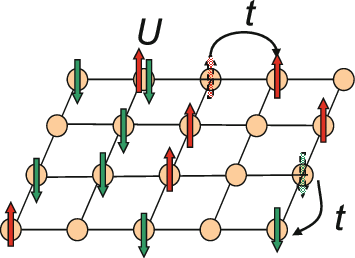
\includegraphics[width=0.5\linewidth]{Praesentation-Bilder/pic2}
	\caption{Zweidimensionales Gitter mit Elektronen}
	\label{fig:pic2}
\end{figure}

\pause
\begin{equation*}\label{Hubbard_standard}
H = -t\sum_{\langle ij\rangle,\sigma}\left( c_{i\sigma}^\dag c_{j\sigma} + c_{j\sigma}^\dag c_{i\sigma}\right) + U \sum_{i}n_{i\uparrow}n_{i\downarrow}
\end{equation*}
\end{frame}

\begin{frame}
\frametitle{Basis des Hubbard-Modells}
Zustand eines Gitterplatzes:\\
\[ \ket{0},\; \ket{\uparrow},\; \ket{\downarrow}\; \text{oder} \; \ket{\uparrow\downarrow}\]\pause
\begin{block}{Problem:}
Insgesamt $ 4^L $ mögliche Zustände
\end{block}\pause
\[ H=\left( \begin{array}{ccc}
H_{N=0}  & 0 & 0\\
0 & H_{N=1} & 0\\
0 & 0 & H_{N=2}\\
\end{array}\right)  \]
$ \Rightarrow $Aufteilung der Basis möglich
\end{frame}

%\begin{frame}
%\frametitle{Impuls-Basis}
%Diagonalisierter hopping-Term:
%\[ H_0 = \sum_{\boldsymbol{k} \sigma} \epsilon_{\boldsymbol{k}} c_{\boldsymbol{k}\sigma}^\dag c_{\boldsymbol{k}\sigma} \]
%Fourier-transformierte Operatoren:
%\[ c_{\boldsymbol{k}\sigma} = \frac{1}{\sqrt{N}}\sum_{j} e^{i\boldsymbol{k}\boldsymbol{R}_j} c_{j\sigma}, \qquad c_{\boldsymbol{k}\sigma}^\dagger = \frac{1}{\sqrt{N}}\sum_{j} e^{-i\boldsymbol{k}\boldsymbol{R}_j} c_{j\sigma}^\dagger \]
%Impulszustand:
%\[ \ket{a(k)} = \frac{1}{\sqrt{N_a}}\sum_{r=0}^{N-1}e^{-ikr}T^r\ket{a} \]
%\end{frame}

\subsection[DMFT]{Dynamical Mean Field Theory}
\begin{frame}
\frametitle{Dynamical Mean Field Theory}
\begin{figure}[h!]
	\centering
	\includegraphics[width=0.6\linewidth]{Praesentation-Bilder/DMFT}
	\caption{Grundlegende Idee der DMFT \cite{Georges}}
	\label{fig:dmft}
\end{figure}\pause
%Die Selbstkonsistenz-Bedingung muss erfüllt sein
\[ G_\sigma(\omega) = \frac{1}{N}\sum_{\boldsymbol{k}}G_{\boldsymbol{k}\sigma}(\omega) = \frac{1}{N}\sum_{\boldsymbol{k}} \frac{1}{\omega + \mu - \epsilon_{\boldsymbol{k}} - \Sigma_{\boldsymbol{k}\sigma}(\omega)} \]
\[ \Sigma_{\boldsymbol{k}\sigma}(\omega) = G_{0\boldsymbol{k}\sigma}^{-1}(\omega)- G_{\boldsymbol{k}\sigma}^{-1}(\omega) \]
\end{frame}

\begin{frame}
\frametitle{Anderson-Impurity-Model}
\begin{figure}[h]
	\centering
	\includegraphics[width=0.3\linewidth]{Praesentation-Bilder/AIM}
	\caption{Geometrie des Elektronen-Bads \cite{Evertz}(Ausschnitt)}
	\label{fig:aim}
\end{figure}
\[ H_{AIM} = \epsilon_d \sum_{\sigma} d_{\sigma}^\dag d_{\sigma} + Un_{d\uparrow}n_{d\downarrow} + \sum_{\sigma,l}\left( V_l c_{l\sigma}^\dag d_{\sigma} + V_l^* d_{\sigma}^\dag c_{l\sigma}\right) \]
\[ + \sum_{\sigma,l}\epsilon_l c_{l\sigma}^\dag c_{l\sigma} \]
\end{frame}

\begin{frame}
\frametitle{DMFT-Loop}
\begin{align*}
	G_0^{-1}&(\omega)\\
	\downarrow& \qquad \text{least square Anpassung}\\
	G^{-1}_{0_{AIM}}&(\omega)\\
	\downarrow& \qquad \text{löse } H_{AIM}\\
	G&(\omega)\\
	\downarrow& \qquad G_0^{-1}(\omega)=\omega+\mu-G(\omega)/2\\
	G_0^{-1}&(\omega)\\
	\circlearrowright&\qquad \text{wiederhole bis }G(\omega) \text{ konvergiert}
\end{align*}
\end{frame}

\begin{frame}
\frametitle{Bethe-Gitter}
\begin{figure}
	\centering
	\includegraphics[width=0.45\linewidth]{Praesentation-Bilder/Bethe}
	\caption{Bethe-Gitter \cite{Wikipedia}}
	\label{fig:bethe}
\end{figure}
\[ \rho_0(\omega) = \frac{\sqrt{4t^2-\omega^2}}{2\pi t^2} \]
\end{frame}

\subsection[Spektralfunktion \&\\Green'sche Funktion]{Spektralfunktion \& Green'sche Funktion}
\begin{frame}
\frametitle{Spektralfunktion \& Green'sche Funktion}
Spektralfunktionen stellen Materialeigenschaften grafisch dar
\[ A(\omega) =\sum_{m}\abs{\bra{\psi_m}B\ket{\psi_0}}^2\delta\left( \omega-(\lambda_m-\lambda_0)\right) \]
Die Spektralfunktion lässt sich einfach aus der Green'schen Funktion berechnen
\[ A(\omega)= \lim\limits_{\eta \rightarrow 0}\,-\frac{1}{\pi}\Im\left[ G(\omega+i\eta)\right]  \]
%\begin{block}{Erinnerung}
%	\[ \lim\limits_{\eta \rightarrow 0}\,-\frac{1}{\pi}\Im\left[ \frac{1}{x+i\eta}\right]  = \delta(x) \]
%\end{block}
Diese lautet für die Zustandsdichte
\[ G(\omega) = \frac{\sum_{m}\big| \bra{\psi_m}c^\dagger_i\ket{\psi_0}\big| ^2}{\omega +\lambda_0 -\lambda_m }  + \frac{\sum_{n}\big| \bra{\psi_n}c_i\ket{\psi_0}\big| ^2}{\omega + \lambda_0 +\lambda_n} \]
\end{frame}

\subsection{Lanczos}
\begin{frame}
\frametitle{Lanczos-Verfahren (exakte Diagonalisierung)}
\begin{block}{Problem:}
Matrix A ist zu groß um direkt diagonalisiert/ gespeichert zu werden
\end{block}\pause
%Krylov-Unterraum:
%\[ \ket{\phi_n} = A^n\ket{\phi_0} \Leftrightarrow \ket{\phi_n} = A\ket{\phi_{n-1}} \]
\[ A\ket{\phi_j} = \beta_{j-1}\ket{\phi_{j-1}}+\alpha_j\ket{\phi_j}+\beta_{j}\ket{\phi_{j+1}} \]
Transformation von $ A $ in den Unterraum
\[ Q^TAQ = T \Leftrightarrow AQ = QT \]
\[ Ty=\lambda y \Rightarrow A(Qy)=\lambda(Qy) \]
\[ T = \left( {\begin{array}{cccc}
	\alpha_1 & \beta_1 & & \\
	\beta_1  &\alpha_2 & \beta_2 & \\
	& \beta_2 & \alpha_3 & \beta_3\\
	& &\beta_3 &\alpha_4\\
	\end{array}}\right)  \]
%\[ \Rightarrow A\ket{\phi_j} = \beta_{j-1}\ket{\phi_{j-1}}+\alpha_j\ket{\phi_j}+\beta_{j}\ket{\phi_{j+1}} \]
\end{frame}

%\begin{frame}
%\frametitle{Lanczos-Verfahren}
%\[ A\ket{\phi_j} = \beta_{j-1}\ket{\phi_{j-1}}+\alpha_j\ket{\phi_j}+\beta_{j}\ket{\phi_{j+1}} \]
%\begin{itemize}
%	\item starte mit $ \ket{\phi_j} $
%	\item berechne $ A\ket{\phi_j} \rightarrow \ket{\phi_{j+1}^{\prime\prime\prime}}$
%	\item (wenn $ j > 0 $)$\;\ket{\phi_{j+1}^{\prime\prime\prime}} - \beta_{j-1}\ket{\phi_{j-1}} \rightarrow \ket{\phi_{j+1}^{\prime\prime}} $
%	\item erhalte $ \alpha_{j} = \bra{\phi_{j}}\ket{\phi_{j+1}^{\prime\prime}} $
%	\item $ \ket{\phi_{j+1}^{\prime\prime}} - \alpha_{j}\ket{\phi_{j}} \rightarrow \ket{\phi_{j+1}^{\prime}} $
%	\item erhalte $ \beta_{j} = \norm{\ket{\phi_{j+1}^{\prime}}}$
%	\item $ \beta_{j}^{-1}\ket{\phi_{j+1}^{\prime}} \rightarrow \ket{\phi_{j+1}}$
%\end{itemize}
%\end{frame}


%\begin{frame}
%\frametitle{Green'sche Funktion}
%Um die Zustandsdichte zu erhalten verwendet man das kombinierte Photoabsorptions und -emissionsspektrum.
%\begin{align*}
%G_{ii}(\omega) = \bra{\psi_0}c_i\frac{1}{(\omega + \lambda_0) I - H}c^\dagger_i\ket{\psi_0} \\+ \bra{\psi_0}c^\dagger_i\frac{1}{(\omega + \lambda_0) I + H}c_i\ket{\psi_0}
%\end{align*}  
%Alternative Schreibweise:
%\[ G(\omega) = \frac{\sum_{m}\big| \bra{\psi_m}c^\dagger_i\ket{\psi_0}\big| ^2}{\omega +\lambda_0 -\lambda_m }  + \frac{\sum_{n}\big| %\bra{\psi_n}c_i\ket{\psi_0}\big| ^2}{\omega + \lambda_0 +\lambda_n} \]
%\end{frame}

\section{Umsetzung}
\begin{frame}
\frametitle{Implementierung - Zustände}
Basisdarstellung:
\[ \ket{L_\uparrow,L-1_\uparrow,\dots,2_\uparrow,1_\uparrow,L_\downarrow,L-1_\downarrow,\dots,2_\downarrow,1_\downarrow} \]
Beispiel:
\[ \ket{\downarrow_1,-_2,\uparrow\downarrow_3}\;\rightarrow \; c^\dagger_{3\uparrow}c^\dagger_{3\downarrow}c^\dagger_{1\downarrow}\ket{0} = \ket{1, 0, 0, 1, 0 , 1} = \ket{37} \]\pause
\begin{block}{Wichtig!}
Fermionen $ \Rightarrow $ Vorzeichenwechsel beachten!
\[ c^\dagger_{1\uparrow}\ket{37} =  c^\dagger_{1\uparrow}c^\dagger_{3\uparrow}c^\dagger_{3\downarrow}c^\dagger_{1\downarrow}\ket{0}=-c^\dagger_{3\uparrow}c^\dagger_{1\uparrow}c^\dagger_{3\downarrow}c^\dagger_{1\downarrow}\ket{0}=-\ket{45}\]
\end{block}
\end{frame}

\begin{frame}
\frametitle{Rechnen mit Impulszuständen}
\begin{block}{Impulszustand}
\[ \ket{a(k)} = \frac{1}{\sqrt{N_a}}\sum_{r=0}^{N-1}e^{-ikr}T^r\ket{a} \]
\end{block}
\[ T^m\ket{a(k)} = e^{ikm}\frac{1}{\sqrt{N_a}}\sum_{r=0}^{N-1}e^{-ik(r+m)}T^{r+m}\ket{a}=e^{ikm}\ket{a(k)} \]
\[ \bra{a(k)}O\ket{b(k)} = \pm\sqrt{\frac{N_a}{N_b}}e^{ikm} \bra{T^ma}O\ket{b} \]
\end{frame}

\begin{frame}
\frametitle{Implementierung - Operatoren}
\begin{block}{Problem}
Der Operator ist häufig zu groß um als Matrix gespeichert zu werden
\end{block}
Beispiel:
\[ H\;\rightarrow\; \mathtt{cx\_vec\: Hamilton(uvec\: Basis,\:cx\_vec\: Psi)}\]


\[ \ket{\psi_{out}} = \sum_{n,m}B^{-1}_{out}\ket{m}\bra{m}OB_{in}\ket{n}\bra{n}\ket{\psi_{in}} \]
\end{frame}

\begin{frame}
\frametitle{Vorgehen beim erstellen der Spektralfunktion}
\begin{enumerate}
	\item suche Grundzustand (in allen k-Unterräumen)
	\begin{itemize}
		\item für jeden k-Unterraum wird ein Lanczos-Verfahren benötigt um den jeweils kleinsten Eigenwert zu finden
	\end{itemize}
\end{enumerate}
\vbox{}\vbox{}\vbox{}\vbox{}\vbox{}\vbox{}\vbox{}\vbox{}\vbox{}\vbox{}\vbox{}\vbox{}
\end{frame}

\begin{frame}
	\begin{figure}
		\centering
		\includegraphics[width=1\linewidth]{Praesentation-Bilder/Ek}
		\caption{Um den Grundzustand zu finden muss man alle k durchgehen}
		\label{fig:ek}
	\end{figure}
	
\end{frame}

\begin{frame}
\frametitle{Vorgehen beim erstellen der Spektralfunktion}
\begin{enumerate}
\item suche Grundzustand (in allen k-Unterräumen)
\begin{itemize}
	\item für jeden k-Unterraum wird ein Lanczos-Verfahren benötigt um den jeweils kleinsten Eigenwert zu finden
	\item für den Grundzustand ein zusätzliches Lanczos-Verfahren um den Vektor in die korrekte Basis zu transformieren\pause
	\item zur Wiederverwendung abspeichern\pause
\end{itemize}
\item der passende Vernichtungsoperator wird auf den Grundzustand angewandt um den Startzustand zu erhalten\pause
\item ein Lanczos-Verfahren wird mit dem Startvektor begonnen um die Green'sche Funktion zu erhalten\pause
\item die Spektralfunktion wird aus der Green'schen Funktion bestimmt\pause
\item die Schritte 2-4 werden auch für den Erzeugungsoperator wiederholt und die Spektralfunktionen werden addiert
\end{enumerate}
\end{frame}

\section{Ergebnisse}
\subsection{Eindimensionales Hubbard-Modell}
%\begin{frame}
%\frametitle{Konvergenz zur analytischen Lösung}
%\begin{figure}[h]
%	\centering
%	\includegraphics[width=0.8\linewidth]{Praesentation-Bilder/konvergenz}
%	\caption{Grundzustandsenergie pro Gitterplatz für U=t=1}
%	\label{fig:konvergenz}
%\end{figure}
%
%\end{frame}

\begin{frame}
\frametitle{Effekt von U auf die Spektralfunktion}
\begin{figure}
	\centering
	\includegraphics[width=0.8\linewidth]{Praesentation-Bilder/plotU}
	\caption{Vergleich zwischen vier Spektralfunktionen}
	\label{fig:l10u1vs5}
\end{figure}

\end{frame}

\subsection{Hubbard-Modell auf Bethe-Gitter}
\begin{frame}
\frametitle{Hubbard-Modell auf Bethe-Gitter}
\begin{figure}
	\centering
	\includegraphics[width=1\linewidth]{Praesentation-Bilder/Selbstkonsistenz}
	\caption{Konvergenz des DMFT-Loops}
	\label{fig:selbstkonsistenz}
\end{figure}

\end{frame}

\begin{frame}
\frametitle{Ergebnisse von Y. Lu et al.}
\begin{figure}
	\centering
	\includegraphics[width=1.\linewidth]{Praesentation-Bilder/Ergebnisse}
	\caption{Spektralfunktion des Hubbard-Modells, mit 3, 11, 31, 101 und 301 Bad-Orbitalen \cite{Lu} (Ausschnitt)}
	\label{fig:ergebnisse}
\end{figure}

\end{frame}

\section[Zusammen-\\fassung]{Zusammenfassung}
\begin{frame}
\frametitle{Zusammenfassung}
\begin{block}{wichtige Erkenntnisse}
\begin{itemize}
\item Hubbard-Modell: beschreibt Übergang von Leiter zu Isolator
\item DMFT: gute Methode, um Vielteilchenprobleme zu lösen
\item Lanczos-Methode: ermöglicht iterative Diagonalisierung von großen Matrizen, wenn man an extremen Eigenwerten interessiert ist
\end{itemize}
\end{block}

\begin{block}{daran kann noch gearbeitet werden}
	\begin{itemize}
		\item weitere Optimierung des Hamilton-Operators, um größere Gitter in endlicher Zeit zu berechnen
		\item verbesserte Anpassung des Impurity-Modells, um den Selbstkonsistenz-Loop auch für größere U und mehr Bad-Orbitale erfolgreich konvergieren zu lassen
	\end{itemize}
\end{block}
\end{frame}

\appendix

\begin{thebibliography}{}
\begin{frame}
\frametitle{Bildquellen}	
	\bibitem{Hubbard}
	M. Machida et al.[CC BY-SA 4.0 (https://creativecommons.org/licenses/by/4.0/)], from Researchgate
	\url{https://www.researchgate.net/figure/A-schematic-figure-of-the-2-dimensional-Hubbard-model-where-t-is-the-hopping-parameter_fig2_323863889}
	
	\bibitem{Georges}
	A.\,Georges {\it Electronic structure of strongly correlated materials from a Dynamical Mean-Field Theory perspective} (IHP Paris, 2006)\\
	\url{http://www-phynu.cea.fr/vie_scientifique/conference/ncorps/pres_georges.pdf} 
	
	\bibitem{Evertz}
	H.\,G.\,Evertz {\it DMRG for Multiband Impurity Solvers} (DMFT: From Infinite Dimensions to Real Materials)
	\url{https://www.cond-mat.de/events/correl18/manuscripts/evertz.pdf}	
\end{frame}	
\begin{frame}
\frametitle{Bildquellen}
\bibitem{Wikipedia}
Kilom691 [CC BY-SA 4.0 (https://creativecommons.org/licenses/by-sa/4.0)], from Wikimedia Commons
\url{https://commons.wikimedia.org/wiki/File:Reseau_de_Bethe.svg}

	\bibitem{Lu}
	Y. Lu, M. Höppner, O. Gunnarsson und M. W. Haverkort {\it Efficient real-frequency solver for dynamical mean-field theory} (PhysRevB.90.085102, 2014)\\
	\url{https://link.aps.org/doi/10.1103/PhysRevB.90.085102}

\end{frame}
\end{thebibliography}




\end{document}